\chapter{Test Bench}
The main idea behind the test bench development was to make it configurable and adaptable. The test bench has been developed parallel to the system and therefore has been redesigned to suit the current needs. It became clear that it has to be able to conduct various tests on any design with adjustable frequencies and not be bound to any design or interface in particular. The general idea of testing a design has been shown in \autoref{fig:test}.

The test bench is responsible for applying the test vectors to the inputs of the UUT and recording the responses. The generation of test patterns, systematic or random, and response evaluation must be repeated for every design tested, therefore this is the responsibility of the test designer. The easiest interface from the users perspective is a PC application acting as the GUI to the test bench. Physical access to the UUT is implemented with hardware description language and, together with the design, implemented into a FPGA. The middleware, responsible for the communication and translation of signals between GUI and physical interface, should support standard communication protocols for data exchange with PC and hardware interface to the FPGA. The rough design draft is shown in the figure \autoref{fig:draft}.\\
 

\begin{figure}[H]
\centering
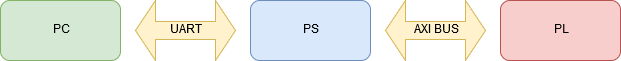
\includegraphics[width=0.65\textwidth]{figures/PCPSPL.png}
\caption{Draft of the test system}
\label{fig:draft}
\end{figure}

\section {Target Architecture}
The target architecture chosen is the Xilinx Zynq SoC (system on Chip). The idea of integrating processors, memories, mixed signal components with RF components in one chip has been known for a long time. Such Application Specific Integrated Circuits (ASICs) are designed to reduce size, to target more secure and faster communication between systems, to lower power consumption and increase reliability. The production cost of a single ASIC is also lower. The main problem of such full custom design is lack of flexibility, high, non-recurring development cost and time. Another important drawback is the lack of compatibility with most of standard applications which speed up the development process and, what comes with it, the time to market. Instead of full-custom ASICs, the semi custom SoCs with programmable logic are gaining on importance. Standard processors connected with Field Programmable Arrays (FPGAs), peripherals and communication systems create an All-Pogrammable-System-on-Chip. The Programmable Logic is ideal for implementing high-speed logic and data flow systems, while Processing System supports operating system and standard software routines.The combination allows the developer to apply any system and easily partition it between hardware and software.

The Xilinx Zynq XC7Z020-1-CLG484 produced in 28nm technology is a SoC solution containing an ARM hardware processor with two cores and an FPGA with 53200 LUTs, 106400 DFFs and 560 KB of Block RAM. It supports all common standard communication interfaces: UART, SPI, CAN, I2C, GigE, GPIO and SDIO . It also allows quick data transfers between Pocessing System (PS) and Programmable Logic (PL) thanks to Xilinx AXI Bus. The full overview of the Zynq architecture is shown in \autoref{fig:Zynq}. The platform suits all needs of the hardware and middleware layer of the test bench.

\begin{figure}[H]
\centering
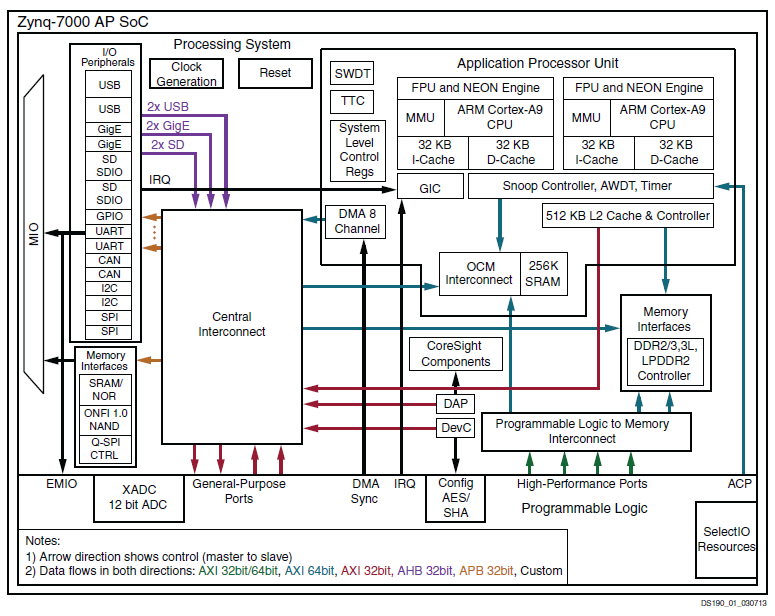
\includegraphics[width=0.65\textwidth]{figures/Zynq.png}
\caption{The Zynq Processing System~\cite{book:ZynqBook}}
\label{fig:Zynq}
\end{figure}

\subsection{FPGA Architecture}

\section{Middleware}
The middleware lays between the user and hardware. All of it's functionality is implemented within one core of the ARM processor available in Zynq. The middleware has direct access only to the modules with AXI interface. The modules are marked yellow in the \autoref{fig:testbench}.

\subsection{AXI Interface}
The history of the Advanced eXtensible Interface (AXI) goes back to year 2003 when it was first introduced as part of the ARM\textsuperscript{\textregistered} Advanced Microcontroller Bus Architecture (AMBA\textsuperscript{\textregistered}). The current version is called AXI4 and was released in 2010 as second version of AXI interface. The number four comes from the fourth version of AMBA, which contains AXI interface. The protocol is supported by many Intellectual Property (IP) producers (not only Xilinx) making the designer learn only one standard of communication. It was developed to standardize the communication between modules in the SoC designs. There are three types or modes of the AXI4:
\begin{itemize}
    \item AXI4 maps the memory of the interface and allows bursts up to 256 data transfers with just single address phase. Writing data to the memory, sends the data directly to the IP,
    \item AXI4-Lite is a light-weight version which offers just memory mapping without the burst capability,
    \item AXI4-Stream doesn't support any address phases. It allows unlimited burst of data. Lack of addresses make it no more considered a memory mapping interface.
\end{itemize}
The protocol works in the master slave system connecting both of them using an AXI Interconnect IP. It applies only to memory mapped versions, since the AXI4-Stream connects master and slave directly or with each other or DMA IP. The AXI Interconnect can service up to 16 masters and 16 slaves. Its main function is the data-width translation, downsizing too big master data packets into smaller slave-compliant bursts or upsizing it. It also does the clock-rate conversion, since both masters and slaves can operate on different clock frequencies. One of the big advantages of the interconnection is the mix support between protocol modes. Moreover the interconnection implements data pipelining for better frequency vs. latency trade-off. Finally it handles priorities in data transitions, making them either concurrent or using programmable priorities.
AXI4 protocol is designed for bidirectional communication, having separate write address, read address, write data, read data and write response channels in memory mapped modes and just data transfer channel in Stream mode. Every Xilinx IP has AXI4 support and there is an easy way of creating custom IPs supporting this protocol~\cite{report:AXI}.

\section{Physical Interface}
The physical interface of the test bench has to supply UUT inputs with test vectors and record responses of the outputs. It is advisable to incorporate the DfT techniques to increase controllability and observability of the UUT. But this step is not required to conduct tests, specially of relatively small modules. The system architecture is shown in \autoref{fig:testbench}.

\begin{figure}[H]
\centering
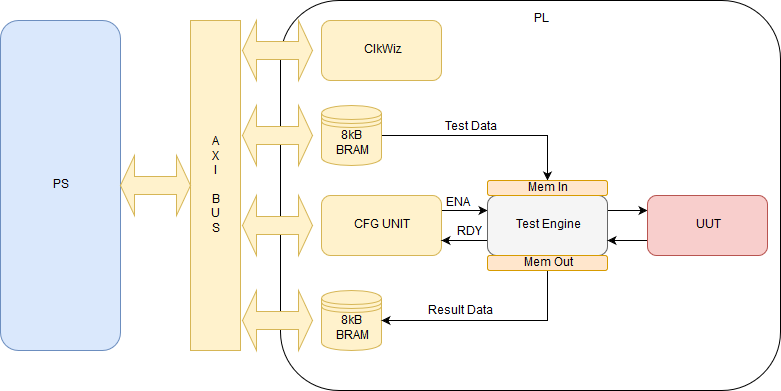
\includegraphics[width=0.65\textwidth]{figures/TestBench.png}
\caption{The Architecture of the Test Bench~\cite{book:ZynqBook}}
\label{fig:testbench}
\end{figure}


\subsection{Data Buffering}
There are two solutions that have been implemented and tested to deliver data to the inputs of the UUT
\begin{itemize}
    \item Direct mapping of the UUT as AXI IP. Every input of the UUT is mapped as different bit in the address space of the AXI interface. Clock input is also mapped in this fashion. The inputs are set to desired values, together with the low level of clock input. To achieve a rising edge of clock, the inputs are held constant for the time of the second transaction, but this time the clock bit is set to one. This scheme results in functional test of the design, without the ability to set the clock to any fix value. It's maximum frequency would be a half of AXI frequency and would amount in 100 MHz. To achieve this frequency, the middleware would have to schedule the bulk transactions of previously buffered data. This idead is showed in \autoref{fig:ver101}
\begin{figure}[h]
\centering
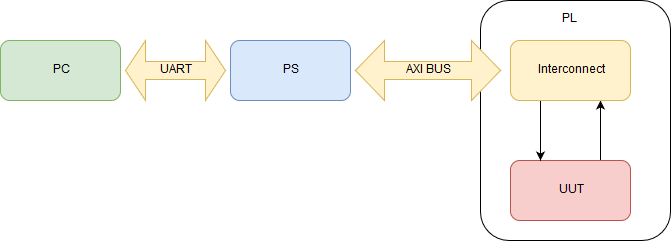
\includegraphics[width=0.65\textwidth]{figures/Version101.png}
\caption{Direct mapping of UUT over AXI interface}
\label{fig:ver101}
\end{figure}
    \item another solution is to buffer the data in the physical layer itself. Buffering limits the amount of data processed during one test run. After all data have been processed, the execution stops and doesn't restart until new data has been written to the memory. For the buffering, the internal Block RAMs have been used. Since they have dual port access, they fit perfectly for the scenario. The dual port capability of a memory implementation means concurrent access to the memory bank from two independent sources. They can be even clocked with two different clocks if necessary.~\cite{report:BRAM}.
    The BRAMs in the test bench are configured to be true dual ports. One port connected to AXI Bus and another port directly to the UUT. Conflicts must never occur because of the state machine implemented. The memory is never accessed by PL and PS simultaneously. The state machine is shown in the \autoref{fig:PSschedule}. There are two instances of the BRAMs, one to supply the stimuli to the UUT, another to store responses. The input BRAM is filled with data. Then the ENA signal starts the test procedure, resulting in: valid responses stored in output BRAM and RDY signal, to indicate the end of the test procedure. The lack of simultaneous accesses from PL and PS would allow to use only one BRAM, connecting one port as the input to the UUT and another port as its output. After the test routine ends, it is possible to switch the connection of one of the ports back to the AXI interface. This solution is more area efficient, but the presence of two BRAMS was determined by a possible extra feature of conducting successive runs with the same stimuli or chaining the output BRAM to be the input of another Test Engine. Hence the two BRAM solution is implemented.
    The drawback of this solution is the maximum frequency of the BRAM, which is 400 MHz. Additionally the clock has to be disabled whenever the data is replaced in the memory.
    \item To overcome the disadvantage of the previous solution, a fully customizable data buffering has been implemented. There are more than one vector stored in one memory word and they get fetched during one memory access. Then the vectors are shifted successively through the UUT. This buffering allows higher frequencies on the UUT side and lower on the memory side. The system was presented in the \autoref{fig:testbench}.
    The depth and width of the BRAMs may be adjusted to suit the testers needs and optimize BRAMs function. They have to be kept equal for both BRAMs at all times because the response vectors have the same length as the test vectors and there are exactly as many vectors stored in one memory word at the input and output. The width of the memory is a very important parameter for frequency multiplication. The $clk_{bram}$ is different then the $clk_{uut}$ and their relation $k$ is strongly connected with the width of BRAM word and the width of the UUT interface showed in~\autoref*{eq:ratio}. 
    \begin{equation}
    k = \frac{clk_{uut}}{clk_{bram}} = \frac{width_{bram}}{width_{uut}}\label{eq:ratio}
    \end{equation}
    For example if the $width_{uut} = 8b$ and the desired test frequency set to $clk_{uut} = 300MHz$ and the BRAM configured to have $width_{bram} = 16b$ then it would have to be clocked with the frequency $clk_{bram} = 150MHz$ to satisfy data throughput. It usually makes sense to set the $width_{bram} > width_{uut}$ to access frequencies higher then $clk_{bram_{max}} = 400 MHz$. The detailed explanation of the origin of this relation can be found in \autoref{ssec:engine}.
\end{itemize}

\subsection{Test Engine}\label{ssec:engine}
The main core of the Test Bench is the Test Engine which feeds the test vectors to the UUT and gathers the response vectors. It consists of two parts:
\begin{itemize}
    \item memory interface which calculates successive addresses for words in the memory bank and stores them in the input register every $clk_{bram}$ cycle. The addresses get incremented by $inc = width_{bram}/8$ due to the bytewise addressing scheme. The memory interface also handles the write back of the response every $clk_{bram}$ cycle from the output register. The number of pipeline stages for memory data read operation has to be taken into account. The number of pipeline stages determines the delay in clock cycles when the information, stored under the address given in the address register, actually gets to the input register of the test engine. The pipeline is used by Xilinx to increase the clock rate of their BRAM modules~\cite{report:BRAM}.
    \item data downsize converter which reads input register and conducts parallel to parallel conversion where the input dimension is the $b=width_{bram}$ and the output dimension is the $u=width_{uut}$. The conversion process takes $k clk_{uut}$ cycles where $k$ is calculated as showed in~\autoref*{eq:ratio}. The Test Engine (\autoref{fig:testeng}) successively shifts the $u$ size test vectors through the design. With each $clk_{uut}$ cycle new data is placed on the input of UUT and new response vector gathered.
    \item the upsize converter recombines the $u$ size responses into $b$ size word with another parallel to parallel conversion. The conversion is done by the shift register with parallel output. The functionality of shift registers is described together with the downsize conversion in the \autoref{subsec:mux}. The test vector and response vector have always the same width $u$, although the number of UUT inputs and outputs may vary. It is necessary to connect the unused ports of the Test Engine to a known constant value.
\end{itemize}
\begin{figure}[h]
\centering
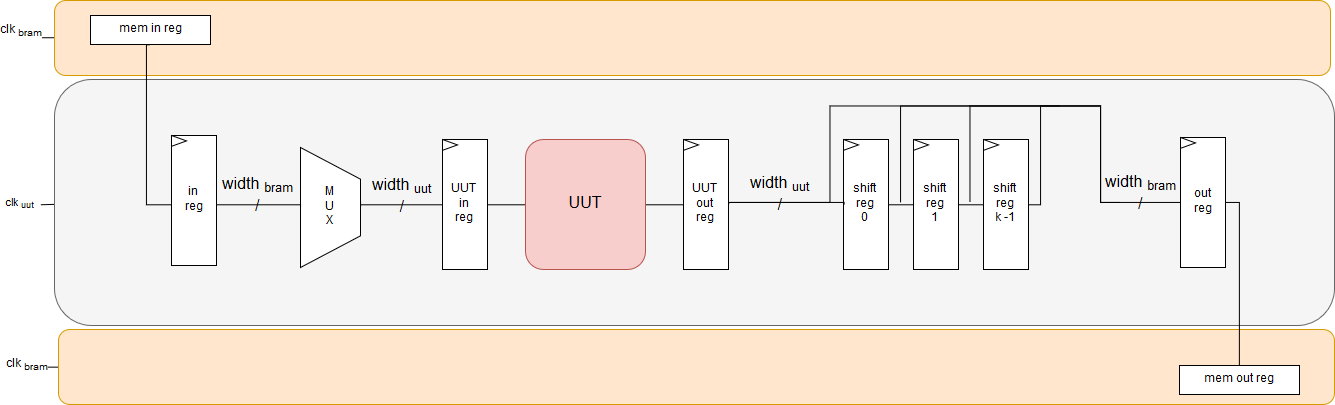
\includegraphics[width=0.65\textwidth]{figures/Test_Engine_complex.png}
\caption{Test engine architecture}
\label{fig:testeng}
\end{figure}

The UUT is surrounded by flip-flops to guaranty, that the tested design is separated from the test engine logic. If it wasn't the case, the test procedure would include the Test Bench design and not only the UUT. Additionally the synthesis tool could combine some of the elements of the converters with the UUT logic. The structure of the Test Engine visible in \autoref{fig:testing} incorporates the idea of pipelining. Large functions are split into smaller atomic operations and the intermediate results are stored between the operations. This concept allows the whole logic to be clocked with higher frequencies, since the path from one register to the next one leads through only few logic gates or LUTs. 

When all buffered test vectores are processed and thereby all responses stored back, the test engine has to unplug the clock from the design. This procedure is conducted by special enable logic which switches on successive pipeline stages and switches them off together with the last valid input data.

\subsubsection{Data multiplexing}label{subsec:mux}
Although the design is pipelined, the memory interface has it's limitations and cannot be possible clocked with the working frequency of the UUT. To overcome this limitation, more than one test vector is stored in one memory word. After the word is fetched, the test vectors are successively shifted through the design. One of the ways to convert wide parallel inputs into series of narrower outputs can be accomplished using big multiplexer (MUX), or rather an array of MUXes. With each tact the converter chooses different part of the longer word to be routed to the output. The solution is shown in \autoref{fig:mux}. Number of MUXes in this solution is always equal to the number of outputs of the converter, with each MUX having as many inputs as the relation $k$. Therefore the solution can be achieved using $u$ $k$-to-1 MUXes.
\begin{figure}[h]
\centering
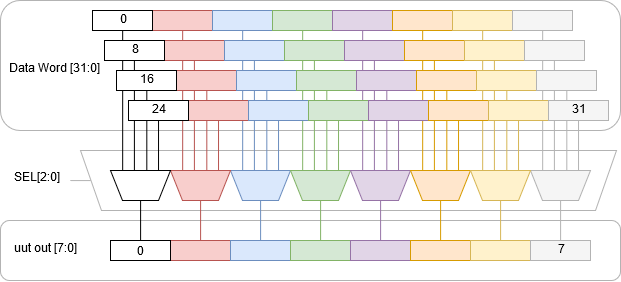
\includegraphics[width=0.65\textwidth]{figures/MUX.png}
\caption{32-to-8 bit converter using 8 4-to-1 MUXes}
\label{fig:mux}
\end{figure}

Another way of conducting a downsize conversion is by splitting it to many parallel to serial conversions. Such conversion can be achieved using shift registers with parallel input and serial output. Shift register consists of more chained registers, so that the output of the previous register is connected to the input of the next one. With each clock cycle the content of each register is copied to the following one. If the last register is connected to the first one, a circular shift is created. The difference between serial and parallel input shift register lays in the way of feeding it with data. In the serial shift register the input is connected to the first register and travels through all of the registers until it gets propagated to the last one. In the parallel input shift register all of the registers are written at once and shifted out one by one. The number of following registers is called the $depth$ of the shift register. With each cycle new vector occurs at the output until all vectors are processed. Then the shift register is loaded with all bits at once and the shifting starts over. The parallel input of shift register requires multiplexing to indicate whether the shift or write operation is going to happen. The shift registers can also have parallel output, meaning that all registers are read at once. The number of 2-to-1 MUXes needed for parallel input shift register is equal to, the depth of the shift register minus one, multiplied by its width. In the proposed solution there is a need of $(b-u)$ 2-to-1 MUXes and extra $k-1$ number of registers to create the shift register. The advantage of this solution are small MUXes with smaller delays, but the hardware overhead is significant. The shift register solution is shown in \autoref{fig:shift}.

\begin{figure}[h]
\centering
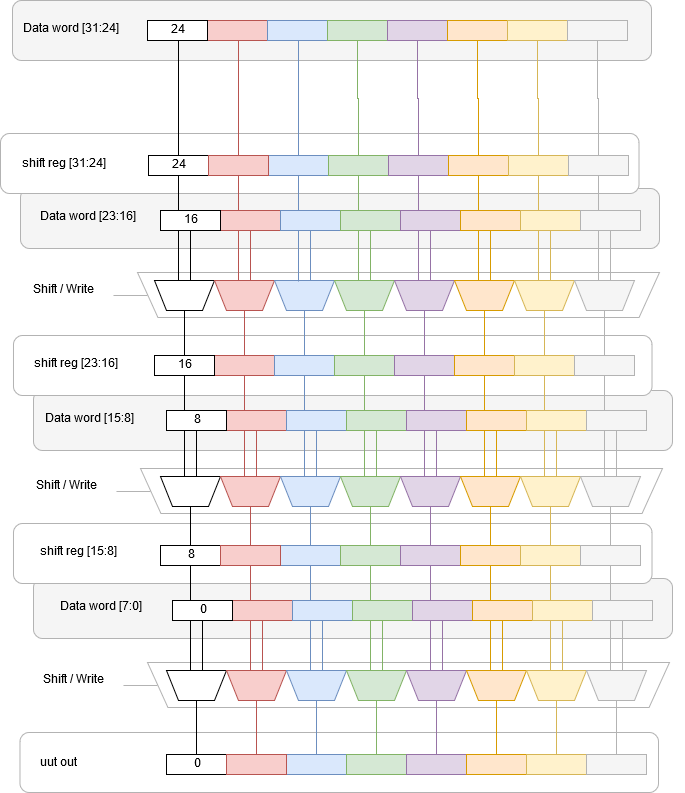
\includegraphics[width=0.65\textwidth]{figures/Shift_2.png}
\caption{32-to-8 bit converter using parallel input shift register and 24 2-to-1 MUXes}
\label{fig:shift}
\end{figure}

To provide the desired conversion each method involves different number of MUXes, therefore different complexity and delay. To compare both solutions, they need to be split into basic multiplexers. Assuming that every multi-input MUX can be broken into cascade of 2-to-1 MUXes, the comparison between the two methods is possible. The breaking method is shown in \autoref{fig:cascade}.

\begin{figure}[h]
\centering
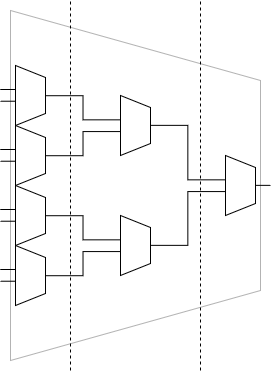
\includegraphics[width=0.25\textwidth]{figures/cascade.png}
\caption{Breaking of 8-to-1 MUX into several 2-to-1 MUXes}
\label{fig:cascade}
\end{figure}

Let's consider an $i$-to-1 MUX. Looking from the right-hand side of the \autoref{fig:cascade} the first cascade has always only one MUX. The next one has 2, and the next one 4. There are always twice as many MUXes in the next step as there were in the previous one. These values are terms of the geometric progression with common ratio $q=2$. The number of 2-to-1 MUXes needed to split an $i$-to-1 MUX into cascades is the sum $S_n$ of all $n$ terms of the progression starting with $a_1=1$ and ending with $a_n=\frac{i}{2}$. The \autoref*{eq:nth} can be used to calculate the number of terms and the \autoref*{eq:sum} the sum of the progression. After rearranging the terms in \autoref*{eq:nth} for $n$ and substituting it with given values, the \autoref*{eq:nthres} shows the number of terms in the progression and therefore the number of cascades of MUXes.
\begin{subequations}
\begin{align}
    a_n&=a_1\cdot q^{n-1}\label{eq:nth}\\
    \frac{a_n}{a_1} &=  q^{n-1}\\
    n &= \log_q \frac{a_n}{a_1}+1\\
    n &= \log_2 i\label{eq:nthres}
\end{align}
\end{subequations}
Using the \autoref*{eq:sum} the sum of the progression and therefore the sum of all MUXes is calculated in \autoref*{eq:sumres}.
\begin{subequations}
\begin{align}
    S_n&=a_1\cdot\frac{1-q^{n}}{1-q}\label{eq:sum}\\
    S_n&=\frac{1-2^{\log_2 i}}{1-2}\\
    S_n&=i-1\label{eq:sumres}
\end{align}
\end{subequations}

To compare both converting solutions, the one with multi-input MUXes has to be broken into cascades of 2-to-1 MUXes. There were $u$ $k$-to-1 MUXes needed in the first solution. Using the \autoref*{eq:sumres} the number of 2-to-1 MUXes needed for this solution is $u(k-1)$. The second solution required $(b-u)$ MUXes, which can be calculated using \autoref*{eq:ratio} as $(uk-u)=u(k-1)$. The number of 2-to-1 MUXes in both solutions is the same, therefore the solution without shift registers is better, because of smaller hardware overhead and is used in the test bench.

\subsection{Configurable Clock}
One of the crucial tasks of the test bench is the ability to test the design with different frequencies. The frequency has to be dynamically adjustable and stable at all times. The dynamical synthesis of the clock is possible thanks to Mixed-Mode-Clock-Manager (MMCM)...

\section{Graphical User Interface}

\begin{figure}[h]
\centering
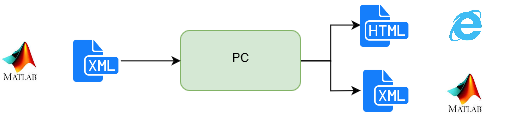
\includegraphics[width=0.25\textwidth]{figures/PC.png}
\caption{Graphical User Interface}
\label{fig:gui}
\end{figure}

\section{Experimental vs. Theoretical parameters}
To test the limits of the Test Bench, and therefore be able to estimate the maximal working frequency for tests, a simple array of NOR gates have been used as UUT. The implementation of one gate in the FPGA takes only one LUT and the logic delay is only X us. For more inputs, there are more LUT needed, but there will always be just one LUT between two registers. If the LUT is not placed far away from the Test Bench it is safe to assume, that the longest path lays somewhere in the rest of the Test Bench. The following table shows the maximum frequency values reported by Vivado IDE. All paths leading from and to the configuration unit are ignored, since those values are treated by the Test Bench as constants and change only off-line.

Another table shows the results during the real test after implementation.

It is visible that the reported values are lower than the real ones. This phenomenon has been described in \ref{PetrPfeifer}.